\chapter{DINOv3 e Architettura del Classificatore}
\label{chap:architettura}

\section{Vision Transformer e Paradigma DINO}
\label{sec:arch_vit}

\subsection{Fondamenti del Vision Transformer}
L'architettura \textit{Vision Transformer} (ViT)~\cite{dosovitskiy2020image} adatta il meccanismo di auto-attenzione (\textit{self-attention})~\cite{vaswani2017attention} alla visione artificiale. Un'immagine d'ingresso $I \in \mathbb{R}^{H \times W \times C}$ viene suddivisa in $N = (H \cdot W) / P^2$ patch bidimensionali disgiunte di lato $P$. Ciascuna patch viene proiettata linearmente in uno spazio latente di dimensione $D$. Alla sequenza risultante è anteposto un token apprendibile ($\mathbf{z}_{\text{CLS}} \in \mathbb{R}^D$), deputato a raccogliere la semantica globale, ed è sommato un vettore di posizione $\mathbf{E}_{\text{pos}} \in \mathbb{R}^{(N+1) \times D}$:
\begin{equation}
    \mathbf{z}_0 = \left[ \mathbf{z}_{\text{CLS}}; \, \mathbf{x}_p^1 \mathbf{E}; \, \dots; \, \mathbf{x}_p^N \mathbf{E} \right] + \mathbf{E}_{\text{pos}}
\end{equation}
La sequenza attraversa $L$ blocchi di \textit{Transformer Encoder}, composti da strati alternati di \textit{Multi-Head Self-Attention} (MHSA) e \textit{Multi-Layer Perceptron} (MLP), preceduti da normalizzazione di strato (\textit{LayerNorm}):
\begin{align}
    \mathbf{z}'_\ell &= \text{MHSA}(\text{LN}(\mathbf{z}_{\ell-1})) + \mathbf{z}_{\ell-1}, \quad \ell = 1, \dots, L \\
    \mathbf{z}_\ell &= \text{MLP}(\text{LN}(\mathbf{z}'_\ell)) + \mathbf{z}'_\ell
\end{align}
In ciascuna delle $h$ teste, l'attenzione opera con dimensione $d_k = D / h$ mediante prodotto scalare scalato:
\begin{equation}
    \text{Attention}(\mathbf{Q}, \mathbf{K}, \mathbf{V}) = \text{Softmax}\left( \frac{\mathbf{Q} \mathbf{K}^\top}{\sqrt{d_k}} \right) \mathbf{V}
\end{equation}
Questo meccanismo offre un campo recettivo globale fin dal primo strato, correlando elementi visivi anche a grande distanza nell'immagine.

\subsection{Pre-addestramento auto-supervisionato in DINOv3}
Privo dell'inductive bias convoluzionale, ViT richiede ampi volumi di dati per apprendere rappresentazioni visive robuste. I modelli DINO~\cite{caron2021emerging,oquab2023dinov2,simeoni2025dinov3} superano questo vincolo mediante auto-supervisione su larga scala: in DINOv3 l'addestramento impiega il corpus LVD-1689M (circa 1.7 miliardi di immagini).

\begin{figure}[htbp]
\centering
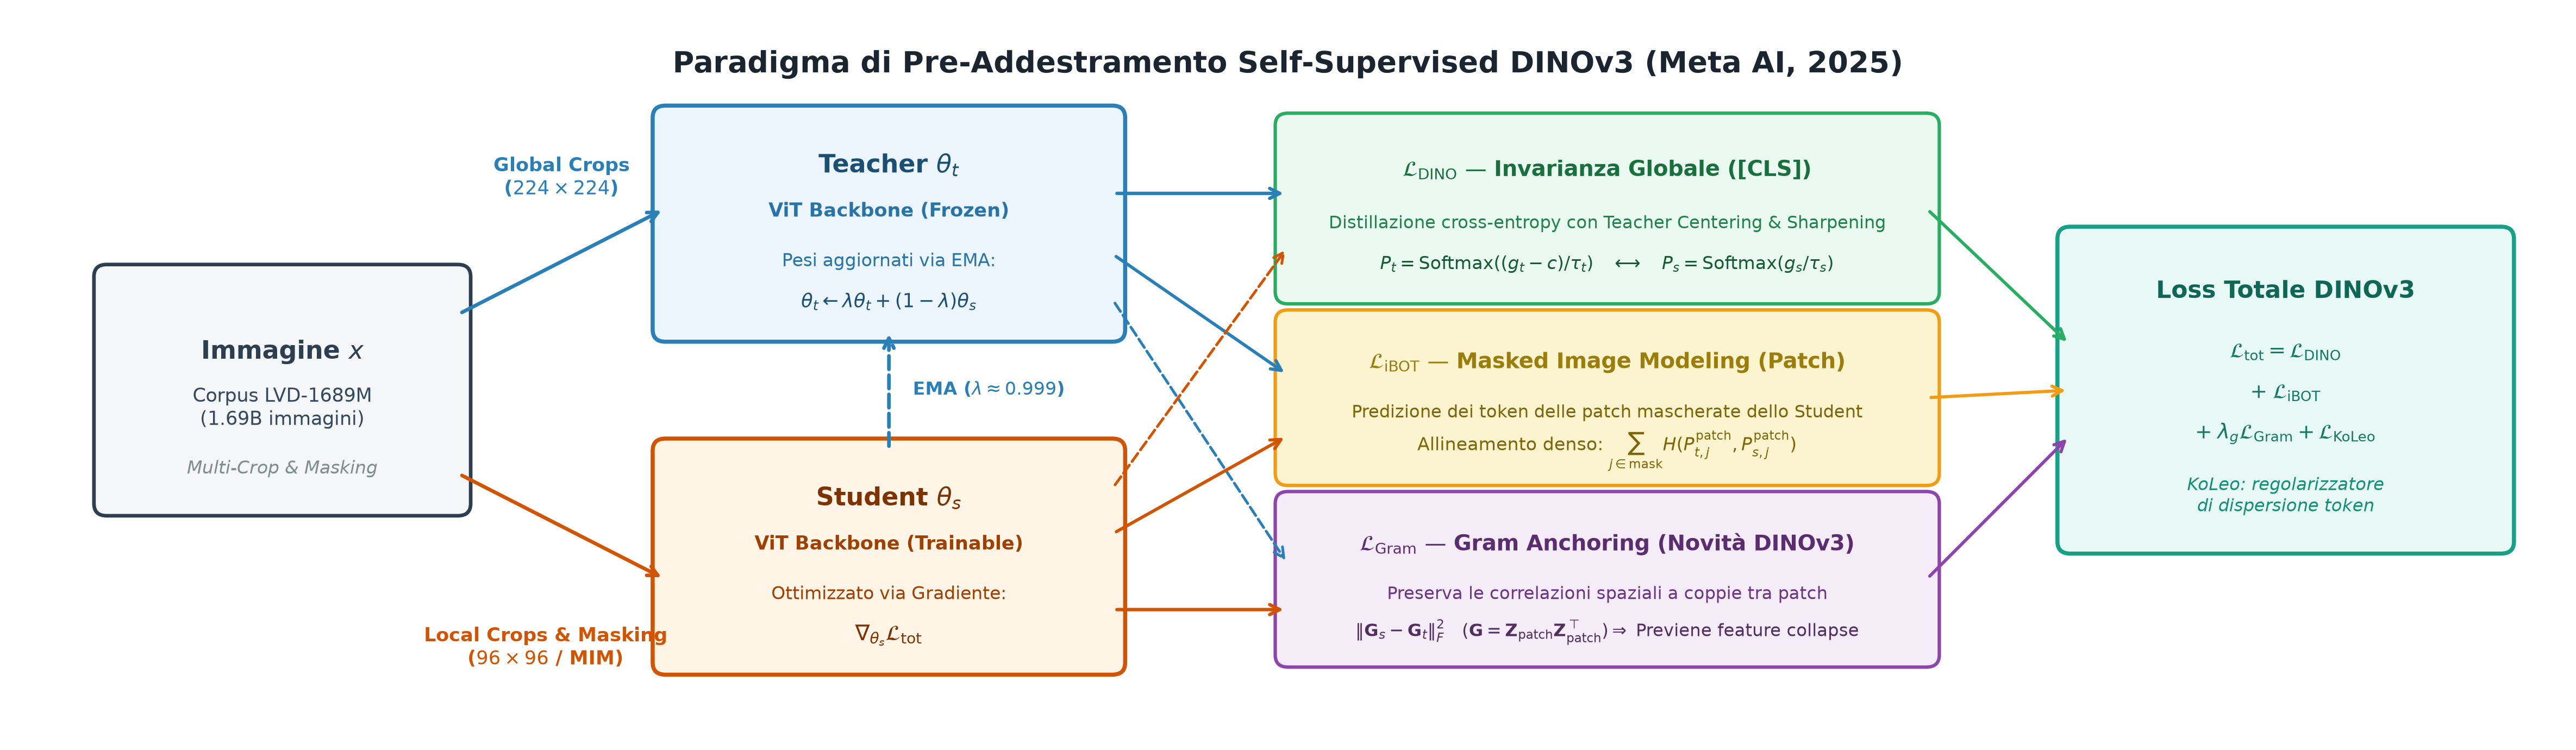
\includegraphics[width=0.92\textwidth]{figure/schema_dino_pretraining.png}
\caption{Architettura di pre-addestramento auto-supervisionato DINOv3~\cite{simeoni2025dinov3}. La rete Student è ottimizzata su obiettivi congiunti ($\mathcal{L}_{\mathrm{DINO}}$, $\mathcal{L}_{\mathrm{iBOT}}$, $\mathcal{L}_{\mathrm{Gram}}$, $\mathcal{L}_{\mathrm{KoLeo}}$); la rete Teacher è aggiornata tramite EMA, guidando la distillazione a livello globale ($[\mathrm{CLS}]$) e denso (patch).}
\label{fig:dino_pretraining}
\end{figure}

Il framework si basa su una distillazione tra due reti omologhe (Figura~\ref{fig:dino_pretraining}): una rete \textbf{Student} con parametri $\theta_s$, ottimizzata via gradiente, e una rete \textbf{Teacher} con parametri $\theta_t$, aggiornata per media mobile esponenziale (EMA):
\begin{equation}
    \theta_t \leftarrow \lambda \theta_t + (1 - \lambda) \theta_s, \quad \lambda \in [0.99, 1.0]
\end{equation}
DINOv3 combina tre funzioni di costo principali e un termine di regolarizzazione:
\begin{enumerate}
    \item \textbf{Loss DINO} ($\mathcal{L}_{\mathrm{DINO}}$): cross-entropy sui token $[\mathrm{CLS}]$ tra ritagli globali e locali. L'uscita del Teacher è stabilizzata tramite \textit{centering} (sottrazione della media empirica dei logit) e \textit{sharpening} (temperatura ridotta sul Softmax), inducendo invarianza alle trasformazioni geometriche.
    \item \textbf{Loss iBOT} ($\mathcal{L}_{\mathrm{iBOT}}$): masked image modeling a livello di patch token; lo Student predice le patch mascherate allineandosi alle rappresentazioni dense non mascherate del Teacher.
    \item \textbf{Gram Anchoring} ($\mathcal{L}_{\mathrm{Gram}}$): vincolo caratterizzante di DINOv3 che allinea le matrici di Gram (correlazioni a coppie tra patch) tra Student e Teacher, prevenendo il collasso delle feature dense durante l'ottimizzazione prolungata su scala miliardaria.
    \item \textbf{Regolarizzatore KoLeo} ($\mathcal{L}_{\mathrm{KoLeo}}$): massimizza l'entropia differenziale, distribuendo uniformemente i vettori latenti nello spazio unitario.
\end{enumerate}
Questo schema integrato consente ai token dell'ultimo strato di catturare confini semantici e separare naturalmente l'oggetto in primo piano dallo sfondo, costituendo la premessa per la localizzazione debolmente supervisionata tramite mappe di attivazione.

\section{Backbone ViT-S/16 e Testa Lineare}
\label{sec:arch_linear_probing}

\subsection{Configurazione del backbone}
Nel presente lavoro viene impiegato il checkpoint ViT-S/16 pre-addestrato. I parametri architetturali sono riassunti nella Tabella~\ref{tab:iperparametri_vits16}.

\begin{table}[htbp]
\centering
\small
\begin{tabularx}{\textwidth}{lcX}
\toprule
\textbf{Iperparametro} & \textbf{Valore} & \textbf{Descrizione Operativa} \\
\midrule
\textbf{Dimensione latente ($D$)} & $384$ & Dimensione del vettore di embedding di ciascun token \\
\textbf{Numero di strati ($L$)} & $12$ & Blocchi sequenziali di Transformer Encoder \\
\textbf{Teste di attenzione ($h$)} & $6$ & Numero di teste nel modulo Multi-Head Self-Attention \\
\textbf{Dimensione per testa ($d_k$)} & $64$ & Spazio di proiezione di ciascuna testa ($384 / 6$) \\
\textbf{Dimensione patch ($P$)} & $16$ & Risoluzione spaziale di ciascuna patch ($16 \times 16$ px) \\
\textbf{Numero di parametri} & $\approx 22\text{ M}$ & Complessità parametrica complessiva del backbone \\
\bottomrule
\end{tabularx}
\caption{Parametri architetturali del backbone DINOv3 ViT-S/16.}
\label{tab:iperparametri_vits16}
\end{table}

\subsection{Linear Probing con backbone congelato}
Per preservare lo spazio latente pre-addestrato ed evitare il \textit{catastrophic forgetting}, il backbone è mantenuto a pesi congelati ($\nabla_{\theta_{\text{backbone}}} \mathcal{L} = 0$).
Sul token globale $\mathbf{z}_{\text{CLS}}^{(L)} \in \mathbb{R}^{384}$ dell'ultimo strato è innestata una testa di classificazione lineare preceduta da Dropout ($p = 0.3$):
\begin{equation}
    \hat{\mathbf{y}} = \mathbf{W} \cdot \text{Dropout}(\mathbf{z}_{\text{CLS}}^{(L)}) + \mathbf{b}
\end{equation}
dove $\mathbf{W} \in \mathbb{R}^{57 \times 384}$ mappa i descrittori latenti sulle $57$ classi del dataset e $\mathbf{b} \in \mathbb{R}^{57}$ è il vettore di bias.

\begin{figure}[htbp]
\centering
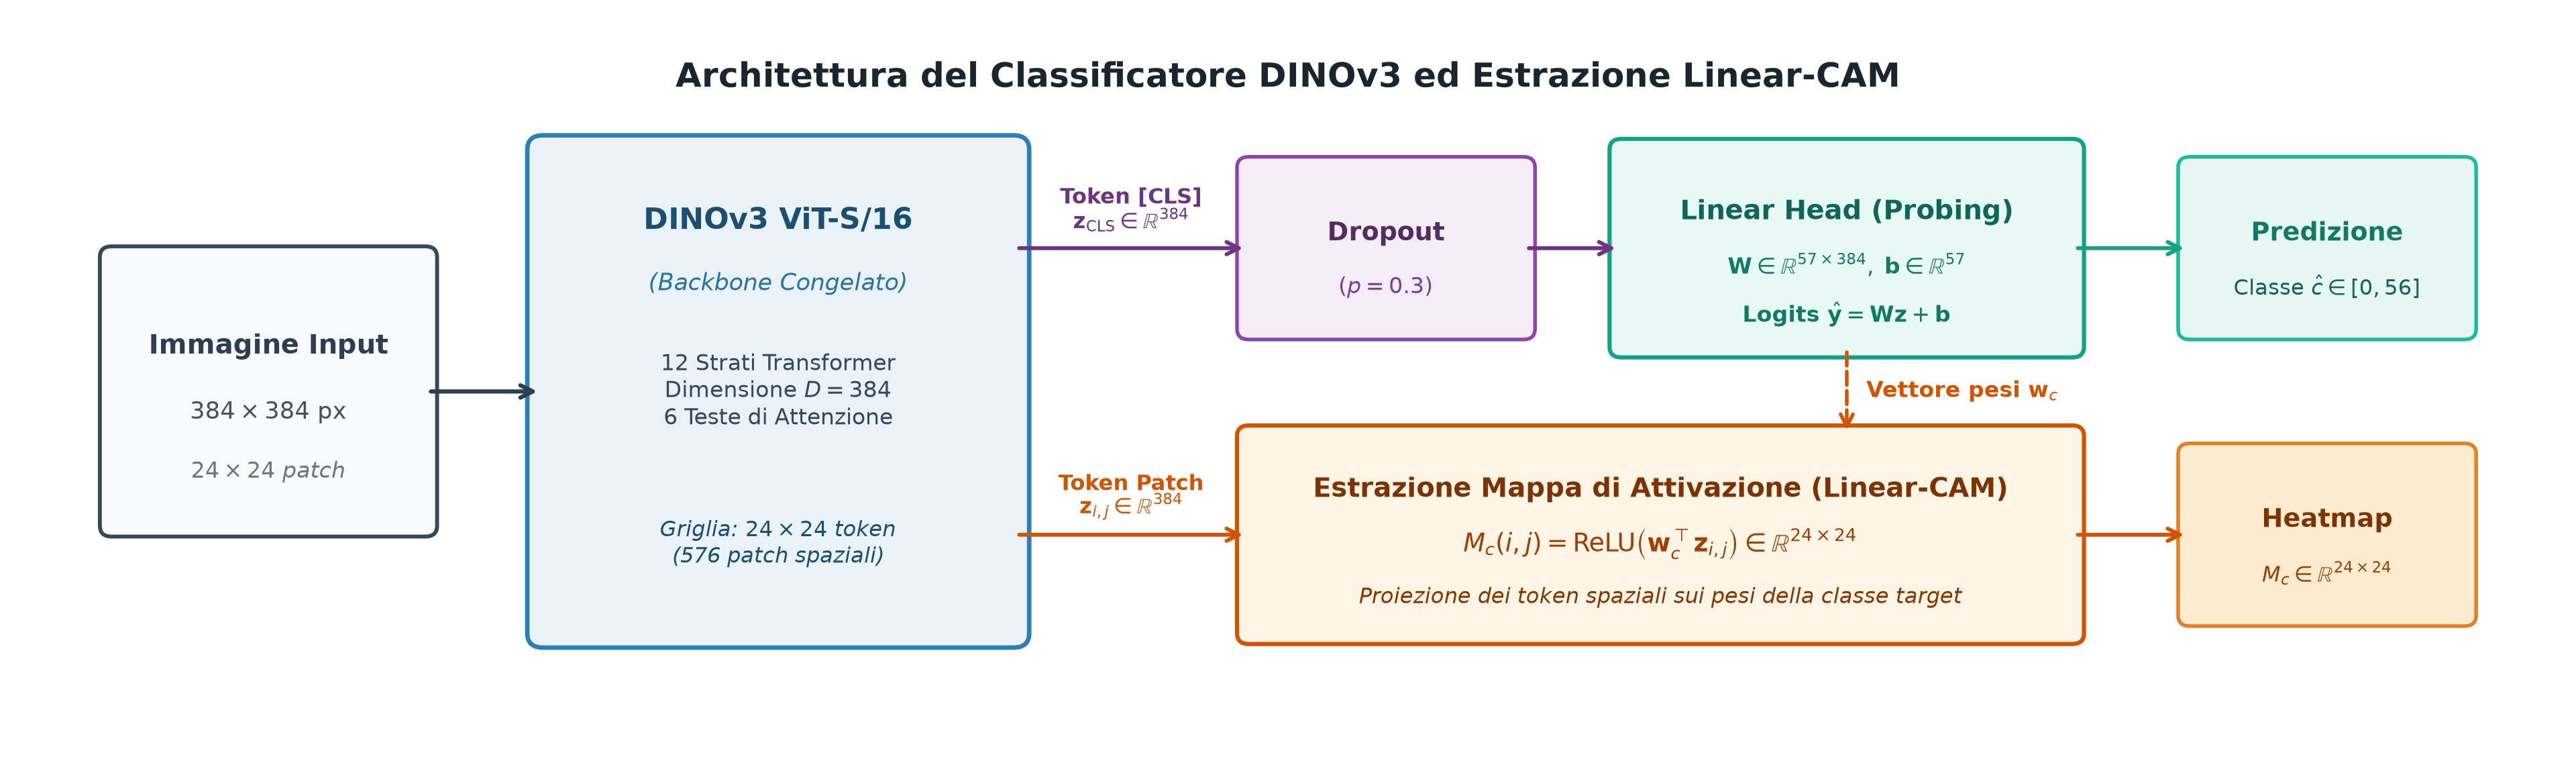
\includegraphics[width=0.88\textwidth]{figure/architettura_classificatore.png}
\caption{Flusso computazionale del classificatore: il backbone ViT-S/16 congelato fornisce sia il token $[\text{CLS}]$ per la predizione di classe (ramo superiore), sia i token di patch impiegati per l'attribuzione Linear-CAM (ramo inferiore).}
\label{fig:architettura_classificatore}
\end{figure}

La linearità della testa fa sì che ciascuna riga $\mathbf{w}_c \in \mathbb{R}^{384}$ della matrice $\mathbf{W}$ corrisponda alla direzione prototipo per la classe $c$. Questa proprietà consente di valutare direttamente l'attivazione locale proiettando $\mathbf{w}_c$ sui singoli token di patch.

\section{Discretizzazione in Patch e Risoluzione Spaziale}
\label{sec:arch_risoluzione}
A risoluzione d'ingresso $H = W = 384$ pixel e lato patch $P = 16$, l'immagine viene suddivisa in una griglia regolare $24 \times 24$, per un totale di $N = 576$ token spaziali oltre al token $[\text{CLS}]$. Ogni cella $(i, j)$ corrisponde a un'area di $16 \times 16$ pixel.
Nei soggetti a scala ridotta (Tier Tiny, area relativa $3\% - 7\%$), il target copre appena $17-40$ celle; in tale intervallo, l'interpolazione continua e la sogliatura operano in prossimità del limite di risoluzione della griglia, aumentando la sensibilità a dispersioni di salienza sullo sfondo.

\section{Metodi di Attribuzione per la Localizzazione Debole (WSOL)}
\label{sec:arch_wsol_cenni}
La combinazione tra i token spaziali di DINOv3 e la testa lineare permette di calcolare quattro mappe di salienza continua $M_c(i, j) \in \mathbb{R}^{24 \times 24}$ per la classe predetta $c$:
\begin{enumerate}
    \item \textbf{Linear-CAM (pesi di classe)}~\cite{zhou2016learning}:
    \begin{equation}
        M_{\text{Linear}}(i, j) = \text{ReLU}\left( \mathbf{w}_c^\top \mathbf{z}_{i, j} \right)
    \end{equation}
    dove $\mathbf{w}_c$ è il vettore dei pesi della classe $c$ e $\mathbf{z}_{i, j}$ è l'embedding del token in $(i, j)$.
    \item \textbf{DINO Self-Attention}:
    \begin{equation}
        M_{\text{Attn}}(i, j) = \frac{1}{h} \sum_{k=1}^h \mathbf{A}_{k}^{(L)}[\text{CLS}, \, (i, j)]
    \end{equation}
    ovvero l'attenzione del token $[\text{CLS}]$ verso i token di patch all'ultimo strato.
    \item \textbf{Eigen-CAM (decomposizione spettrale)}~\cite{muhammad2020eigen}:
    \begin{equation}
        M_{\text{Eigen}}(i, j) = \mathbf{V}_1^\top \mathbf{z}_{i, j}
    \end{equation}
    proiettando le feature spaziali sul primo autovettore principale $\mathbf{V}_1$ ricavato via SVD.
    \item \textbf{Grad-CAM (gradiente sui tensori intermedi)}~\cite{selvaraju2017grad}:
    \begin{equation}
        M_{\text{Grad}}(i, j) = \text{ReLU}\left( \sum_{d=1}^D \alpha_d^c \cdot z_{i, j, d} \right), \quad \alpha_d^c = \frac{1}{N} \sum_{i, j} \frac{\partial \hat{y}_c}{\partial z_{i, j, d}}
    \end{equation}
\end{enumerate}
Il confronto quantitativo tra queste formulazioni è presentato nel Capitolo~\ref{chap:wsol}.
